Some election audits have benefited from a one-and-done approach: draw a large sample with high probability of stopping in the first round and usually avoid a second round altogether. This is appealing for two reasons. Firstly, rounds have some overhead in time and effort. Thus the workload (cost and time) of an audit grows not just with the number of ballots sampled but also with the number of rounds. Secondly, smaller first round sizes give a higher probability that the result after the first round is misleading in the sense that the true winner is losing by the tally of the sampled ballots. On the other hand, a one-and-done audit may draw more ballots than are necessary. To evaluate the efficiency of various round schedules, we propose a simple workload model. Under this model, our simulation results suggest that slightly smaller round sizes give lower average workload. 

We begin with the simple assumption that part of the workload grows linearly with the number of ballots, giving us the per ballot cost parameter $c_{b}$. It is less clear how cost is related to the number of rounds, but we propose a simple model in which the round cost is also linear, with constant per round cost $c_{r}$. This is a reasonable assumption for contests with small margin in which all or nearly all ballot boxes need to be opened in each round. [@Poorvi, I need help justifying the workload model.]

So for an audit $\mathcal{A}$ with expected number of ballots $E_{b}$ and expected number of rounds $E_{r}$, we get that the cost $C$ of the audit is
\begin{equation}
C(\mathcal{A}) = E_b c_b + E_r c_r
\label{eq:cost}
\end{equation}

Analytical approximation of the expected audit behavior ($E_b$ and $E_r$) is challenging since the number of possible sequences of samples grows exponentially with the number of rounds. 
%A very rough approximation scheme is possible and may be useful when choosing round sizes in practice. We implement such a scheme, available at \cite{software}.
%We will use the more standard approach of simulations to give an example here.
Therefore we again use the standard approach of simulations.

Consider the US state of Michigan. In the 2020 US Presidential contest, Michigan had a margin of $2.8\%$.

We let the per ballot cost be one, $c_b=1$. Then the per round cost $c_r$ tells us the cost of a round as a number of ballots. We begin with an example in which $c_r=10$. That is, we suppose that the overhead of a round is equal to the workload of sampling $10$ ballots.

We now consider a simple round schedule for our example. Each round is selected to give the same probability of stopping, $p$. If the audit does not stop in the first round, we find a round size which, given the sample drawn in the first round, will give a probability of stopping $p$ in the second round. For this round schedule scheme, a one-and-done audit is achieved by choosing large $p$, say $p=.9$ or $p=.95$. For this particular round schedule scheme, computing the expected number of rounds is possible analytically(TODO: I worked it out, just need to add here). Our simulations are then used to estimate the expected number of ballots.

\begin{figure}
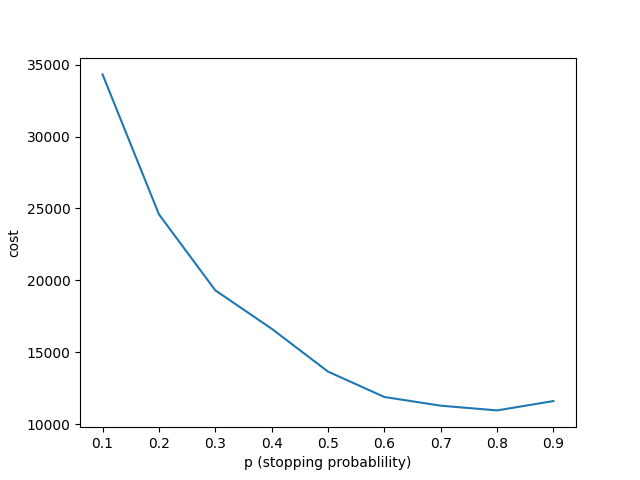
\includegraphics[width=.5\textwidth]{workload.png}
\caption{For cost parameters $c_b=1$ and $c_r=10$, this plot shows the expected cost for various round schedule parameters $p$. Expected cost is found using Equation~\ref{eq:cost} and the average number of ballots and rounds in our simulations as the expected number of ballots and rounds.}
\label{fig:workload}
\end{figure}

The simulation results for our example are given in Figure~\ref{fig:workload}. 
For various round schedules, given by the varying parameters $p$ on the horizontal axis, we see that the average audit cost varies with a minimum at roughly $.8$. In particular, the one-and-done $p=.9$ audits have an average of $zz\%$TODO higher cost than the $p=.8$ audits. Especially for low margin contests, using the cost-minimizing round schedule could translate to significant reduction in cost or savings in time, a particularly important factor given tight certification deadlines.

Without workload measurements from multiple round audits, it is difficult to know an accurate value for $c_r$, and so we also evaluate the simulation results with varying $c_r$. 
For each $c_r$, we find the value of $p$ which minimizes the expected workload as we did in Figure~\ref{fig:workload}. Rather than use the minimum cost estimate among the sparsely sampled points, we fit a quadratic polynomial and use its minimum to get a smoother relationship between $c_r$ and optimal $p$. Figure~\ref{fig:optimal_ps} presents, for varying $c_r$ the round schedule parameter $p$ which minimizes expected workload. 
We observe that for a workload model with no overhead for each round (i.e. $c_r=0$), the optimal round schedule is that with $p=0.72$. As $c_r$ increases, the optimal value of $p$ also increases, up to as much as $p=.9$ for $c_r=10^4$.

Analysis like this can be used to select round schedules for audits. 

% check that report to see if we can at least suggest what might be reasonable

\begin{figure}
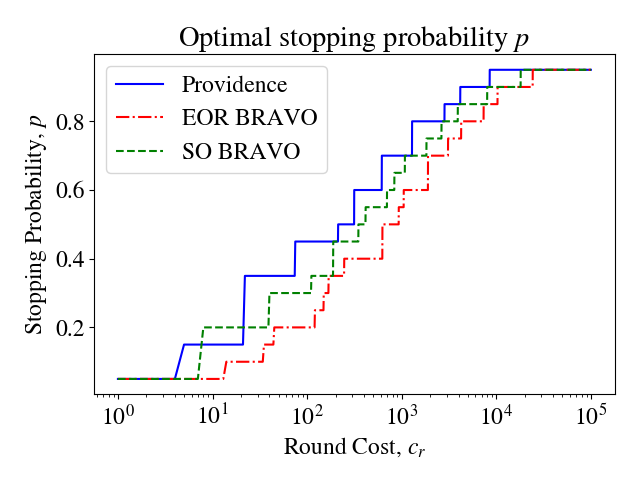
\includegraphics[width=.5\textwidth]{optimal_ps.png}
\caption{The optimal (cost-minimizing) stopping probability $p$ for varying cost model parameters $c_r$. With $c_b=1$, the varying value of $c_r$ can equivalently be thought of as the ratio of the cost of a round to the cost of a ballot.}
\label{fig:optimal_ps}
\end{figure}







